\documentclass[a4paper,11pt]{article}

\usepackage[utf8]{inputenc}
\usepackage[margin=2.7cm]{geometry}
\usepackage{hyperref}
\usepackage{physics}
\usepackage{booktabs}
\usepackage{amssymb}
\usepackage{gensymb}
\usepackage{graphicx}
\usepackage{caption}
\usepackage{subcaption}
\usepackage{xcolor}
\usepackage{listings}
\usepackage{braket}
\usepackage{enumitem}
\usepackage{empheq}
\usepackage{tikz}
\usepackage{adjustbox}
\usetikzlibrary{arrows.meta}

\definecolor{photon}{RGB}{240,200,0}    % jaune / photon
\definecolor{electron}{RGB}{0,160,60}   % vert  / électron
\usetikzlibrary{arrows.meta,angles,quotes,calc,positioning}

\definecolor{kicol}{RGB}{24,95,165}    % blue  -- electron before
\definecolor{kfcol}{RGB}{15,110,86}    % green -- electron after
\definecolor{qcol}{RGB}{153,60,29}     % brown -- phonon
\definecolor{accent}{RGB}{24,95,165}   % titlepage accent rule

\hypersetup{
    colorlinks=true,
    linkcolor=black,
    citecolor=accent,
    urlcolor=accent,
    pdftitle={Beam Propagation Simulation in SiO2},
    pdfauthor={Anatole Cremel--Schlemer}
}

\title{Beam Propagation Simulation in $\mathrm{SiO}_2$}
\author{Anatole CREMEL--SCHLEMER \\ The University of Tokyo}
\date{\today}

\begin{document}

\begin{titlepage}
    \centering
    \vspace*{2cm}
    {\Large\scshape The University of Tokyo\par}
    \vspace{3cm}

    \rule{\linewidth}{0.6mm}\\[0.5cm]
    {\huge\bfseries Beam Propagation Simulation\\[0.3cm] in $\mathrm{SiO}_2$\par}
    \vspace{0.5cm}
    \rule{\linewidth}{0.6mm}\\[2cm]

    \begin{minipage}{0.45\textwidth}
        \begin{flushleft}\large
            \textit{Author}\\
            Anatole \textsc{Cremel--Schlemer}
        \end{flushleft}
    \end{minipage}
    \hfill
    \begin{minipage}{0.45\textwidth}
        \begin{flushright}\large
            \textit{Date}\\
            \today
        \end{flushright}
    \end{minipage}

    \vfill
\end{titlepage}

\tableofcontents
\newpage

\section{Introduction}

Since their invention in the early 80's \cite{fork1981}, femtosecond lasers have rapidly advanced the frontiers of materials science research due to their high peak intensity and outstandingly short temporal resolution.

The ultra-short nature of femtosecond pulses has enabled imaging of ultrafast processes, such as chemical reactions \cite{zewail1994} and the complex energy transfer dynamics between electrons and crystal lattices in solids \cite{shah1996}, whereas the high peak intensity of these pulses allows them to ionise matter and trigger laser-produced plasma (LPP), which emits a variety of spectra, including X-rays \cite{mao2004}.

Studying the dynamics of femtosecond pulses in dielectric media, ranging from the near-UV to the near-infrared, helps clarify the transfer of electromagnetic energy to electrons, followed by electron-lattice interactions that convert energy into heat \cite{mao2004}. However, such studies remain challenging, and some phenomena remain weakly understood for wide-bandgap dielectric materials.

Indeed, these media are transparent under low-intensity irradiation, and when they are irradiated by an intense femtosecond pulse, a cascade of effects begins, ranging from non-linear ionisation occurring within a few femtoseconds to thermal effects occurring on millisecond timescales \cite{bulgakova2010}. Once non-linear ionisation becomes significant, the material loses its transparency, leading to photo-induced damage.

Femtosecond laser processing techniques have an edge over continuous-wave laser machining techniques because of the extremely fast interaction time between the beam and the sample. The damage induced by femtosecond laser pulses is mainly driven by electronic excitation and associated non-linear processes before the material lattice has equilibrated with the excited carriers \cite{mao2004}. This allows for better control over collateral thermal damage and thermal stresses, which are typically associated with continuous laser processing. Also, the non-linear response allows for structural modifications of dielectrics inside the bulk and paves the way for microstructuring that creates subwavelength "voxels" \cite{mao2004}.

The complexity of these nonlinear interactions has spurred extensive research aimed at understanding their fundamental mechanisms and harnessing these properties to develop precision laser processing techniques.

This work presents a simulation of beam propagation in $\mathrm{SiO}_2$ using the nonlinear Schrödinger equation and equations governing electron density evolution. We will explain the physics underlying the model, as well as some of the numerical methods used to solve this complex system.

\section{Excitation of Free Carriers}

Current experimental methods for generating femtosecond lasers in the near ultraviolet range (NUV) remain complex, which limits research on the linear optical transitions of wide bandgap dielectric materials such as $\mathrm{SiO}_2$.

Given these experimental limitations, research has focused mainly on the study of nonlinear absorption processes that generate free carriers in the conduction band. By responding to the electric field, these electrons increase their energy and trigger effects such as avalanche ionization, which modify the optical properties of the material, in particular its absorbance~\cite{mao2004, bulgakova2010}.

In this section, we explain the nonlinear mechanisms responsible for the generation of free carriers, that is, the excitation of electrons from the valence band to the conduction band. In wide bandgap dielectrics, these carriers are central to the light matter interaction, since they are the only way to transfer optical energy to the crystal lattice of the material, which is otherwise transparent to low intensity light.

\subsection{Photoionisation}

\begin{figure}[htbp]
    \centering
    \resizebox{\textwidth}{!}{
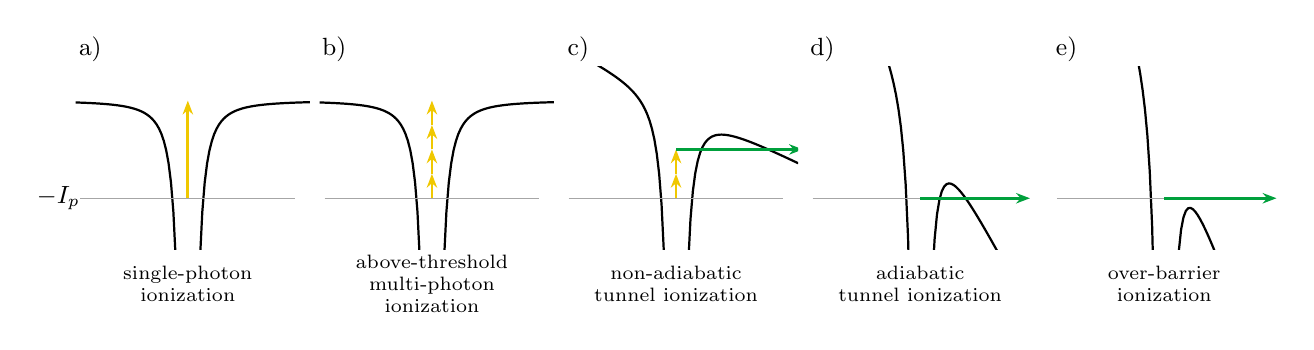
\begin{tikzpicture}[
  scale=0.62,
  well/.style      = {thick, black, line cap=round},
  ipline/.style    = {gray!70, thin},
  photonarr/.style = {photon,   line width=1.0pt, -{Stealth[length=5pt]}},
  elecarr/.style   = {electron, line width=1.1pt, -{Stealth[length=5pt]}},
  tick/.style      = {photon,   line width=1.0pt},
  panellabel/.style= {font=\small},
  regime/.style    = {font=\scriptsize, align=center, text width=2.8cm}
]

% étiquette -Ip (une seule fois, à gauche)
\node[font=\small] at (-2.65,-1) {$-I_p$};

% =====================================================================
% a) SINGLE-PHOTON  (xshift 0) : puits symétrique, flèche pleine
% Paramètre a = 0
% =====================================================================
\begin{scope}[xshift=0cm]
  \clip (-2.3,-2.05) rectangle (2.5,1.7);
  \draw[well] plot[domain=-2.5:-0.1, samples=50] (\x, {-1/(5*\x*\x) + 1});
  \draw[well] plot[domain=0.1:2.5, samples=50] (\x, {-1/(5*\x*\x) + 1});
  \draw[ipline] (-2.2,-1)--(2.2,-1);
  \draw[photonarr] (0,-1)--(0,1);
\end{scope}
\node[panellabel] at (-2.0,2.05) {a)};
\node[regime]     at (0,-2.75)   {single-photon\\ionization};

% =====================================================================
% b) ABOVE-THRESHOLD MPI  (x-shift 5) : même puits, flèche pointillée + rungs
% Paramètre a = 0
% =====================================================================
\begin{scope}[xshift=5cm]
  \clip (-2.3,-2.05) rectangle (2.5,1.7);
  \draw[well] plot[domain=-2.5:-0.1, samples=50] (\x, {-1/(5*\x*\x) + 1});
  \draw[well] plot[domain=0.1:2.5, samples=50] (\x, {-1/(5*\x*\x) + 1});
  \draw[ipline] (-2.2,-1)--(2.2,-1);
  % flèche pointillée
  \draw[photonarr] (0,-1.0)--(0,-0.5);
  \draw[photonarr] (0,-0.5)--(0,-0.0);
  \draw[photonarr] (0,0)--(0,0.5);
  \draw[photonarr] (0,0.5)--(0,1.0);
  

\end{scope}
\node[panellabel] at (3.0,2.05) {b)};
\node[regime]     at (5,-2.75)  {above-threshold\\multi-photon ionization};

% =====================================================================
% c) NON-ADIABATIC TUNNEL  (xshift 10) : barrière large, montée + tunnel
% Paramètre a = 0.1
% =====================================================================
\begin{scope}[xshift=10cm]
  \clip (-2.3,-2.05) rectangle (2.5,1.7);
  \draw[well] plot[domain=-2.5:-0.1, samples=50] (\x, {-1/(5*\x*\x) + 1 - 0.5*\x});
  \draw[well] plot[domain=0.1:2.5, samples=50] (\x, {-1/(5*\x*\x) + 1 - 0.5*\x});
  \draw[ipline] (-2.2,-1)--(2.2,-1);
  % montée multiphotonique (courte, jaune)
  \draw[photonarr] (0,-1.0)--(0,-0.5);
  \draw[photonarr] (0,-0.5)--(0,-0.0);
  % tunnel à travers la barrière (vert, sortie à droite)
  \draw[elecarr] (0,-0)--(2.60,-0);
\end{scope}
\node[panellabel] at (8.0,2.05)  {c)};
\node[regime]     at (10,-2.75)  {non-adiabatic\\tunnel ionization};

% =====================================================================
% d) ADIABATIC TUNNEL  (xshift 15) : barrière plus inclinée, tunnel à -Ip
% Paramètre a = 0.9
% =====================================================================
\begin{scope}[xshift=15cm]
  \clip (-2.3,-2.05) rectangle (2.5,1.7);
  \draw[well] plot[domain=-2.5:-0.1, samples=50] (\x, {-1/(5*\x*\x) + 1 - 1.9*\x});
  \draw[well] plot[domain=0.1:2.5, samples=50] (\x, {-1/(5*\x*\x) + 1 - 1.9*\x});
  \draw[ipline] (-2.2,-1)--(2.2,-1);
  % tunnel horizontal au niveau -Ip
  \draw[elecarr] (0,-1)--(2.25,-1);
\end{scope}
\node[panellabel] at (13.0,2.05) {d)};
\node[regime]     at (15,-2.75)  {adiabatic\\tunnel ionization};

% =====================================================================
% e) OVER-BARRIER  (xshift 20) : barrière abaissée sous -Ip, sortie libre
% Paramètre a = 1.6
% =====================================================================
\begin{scope}[xshift=20cm]
  \clip (-2.3,-2.05) rectangle (2.5,1.7);
  \draw[well] plot[domain=-2.5:-0.1, samples=50] (\x, {-1/(5*\x*\x) + 1 - 2.8*\x});
  \draw[well] plot[domain=0.1:2.5, samples=50] (\x, {-1/(5*\x*\x) + 1 - 2.8*\x});
  \draw[ipline] (-2.2,-1)--(2.2,-1);
  % l'électron passe au-dessus de la barrière supprimée
  \draw[elecarr] (0.0,-1)--(2.30,-1);
\end{scope}
\node[panellabel] at (18.0,2.05) {e)};
\node[regime]     at (20,-2.75)  {over-barrier\\ionization};

\end{tikzpicture}
}
    \caption{Illustration des différents régimes d'ionisation.}
    \label{fig:regimes_ionisation}
\end{figure}

Une forte focalisation conduit à une intensité optique élevée dans le matériau. Cette forte concentration de photons au même endroit augmente la probabilité d'ionisation multiphotonique, un effet non-linéaire~\cite{mao2004}. Plus le champ est intense, plus le potentiel liant l'électron à l'ion est déformé. Au-delà d'un certain seuil d'intensité, la barrière prend une forme triangulaire et devient suffisamment fine pour permettre l'ionisation par effet tunnel. Le paramètre de Keldysh a été introduit pour distinguer entre le régime où domine l'ionisation multiphotonique et celui où domine l'ionisation par effet tunnel~\cite{mao2004}.

Dans le modèle semi-classique, un électron s'échappe à travers une barrière de largeur $l = U_i/e\mathcal{E}$ avec une vitesse $v = \sqrt{2U_i/m}$. Le temps nécessaire pour traverser cette distance est :
\begin{equation}
\tau_{\text{tun}} = \frac{l}{v} = \frac{U_i/e\mathcal{E}}{\sqrt{2U_i/m}} = \frac{\sqrt{2m U_i}}{e\mathcal{E}}
\end{equation}

Le temps caractéristique pendant lequel l'ionisation par effet tunnel peut se produire est donné par $\tau \approx 1/\omega_0$. Le rapport de ces temps est alors :
\begin{equation}
\gamma = \frac{\tau_{\text{tun}}}{\tau} = \omega_0\frac{\sqrt{2m U_i}}{e\mathcal{E}}
\end{equation}

Si le rapport $\gamma \ll 1$, cela signifie que le temps de traversée par effet tunnel est très court comparé au temps d'ionisation. L'effet tunnel est instantané à l'échelle du cycle laser. Le champ se comporte comme un champ quasi-statique. Inversement, si $\gamma \gg 1$, le champ oscille trop rapidement pour permettre à l'électron de traverser la barrière par effet tunnel, l'ionisation nécessite alors une absorption multiphotonique~\cite{bulgakova2010}.

Le taux de photoionisation de Keldysh est défini comme suit :
\begin{equation}
W_{PI}(|\mathcal{E}|) = \frac{2\omega_0}{9\pi}\bigg(\frac{\omega_0m}{\hbar\sqrt{\gamma_1}}\bigg)^{\frac{3}{2}}Q(\gamma,x)\exp(-\alpha\lceil x+1\rceil)
\end{equation}

Avec $\gamma_1 = \frac{\gamma^2}{1+\gamma^2}$, $\gamma_2 = \frac{1}{1+\gamma^2}$ et $x = \frac{2}{\pi}\frac{U_iE(\gamma_2)}{\hbar\omega_0\sqrt{\gamma_1}}$
\begin{equation}
Q(\gamma,x) = \frac{\pi}{2K(\gamma_2)}\sum^\infty_{n=0}\exp \bigg(-n\pi\frac{K(\gamma_1)-E(\gamma_1)}{E(\gamma_2)}\bigg)\Phi\bigg(\frac{\pi}{2}\sqrt{\frac{n+2\lceil x + 1\rceil-2x}{K(\gamma_2)E(\gamma_2)}}\bigg)
\end{equation}

$\Phi$ est la fonction de Dawson $\Phi(z) = e^{-z^2}\int^z_0e^{y^2}dy$ et $K$ et $E$ sont les intégrales elliptiques complètes respectivement de première et deuxième espèce, avec le paramètre $m = k^2$
\begin{align}
K(m) &= \int_0^{\pi/2} [1 - m \sin(t)^2]^{-1/2} dt \\
E(m) &= \int_0^{\pi/2} [1 - m \sin(t)^2]^{1/2} dt
\end{align}

Comme observé dans la référence~\cite{PhysRevB.71.125435}, la filamentation dans la silice fondue se produit typiquement à des intensités autour de $5 \times 10^{13} \text{ W/cm}^2$, où l'ionisation multiphotonique et par effet tunnel contribuent toutes deux de manière significative.

\begin{figure}[htbp]
    \centering
    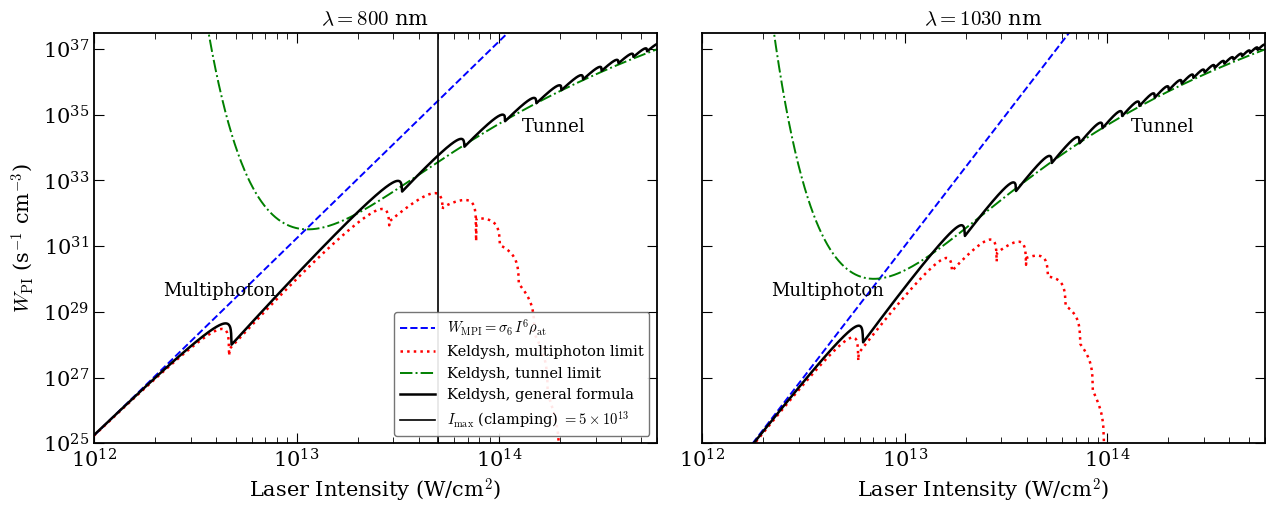
\includegraphics[width=1\linewidth]{sections/téléchargement.png}
    \caption{Le taux de photoionisation $W_{\text{PI}}$ dans la silice fondue ($U_i = 9 \text{ eV}$) est tracé en fonction de l'intensité laser pour $\lambda = 800 \text{ nm}$ et $\lambda = 1030 \text{ nm}$. La ligne solide noire représente la formule générale complète de Keldysh, tandis que les lignes pointillées rouges et tiret-point vert montrent ses asymptotes analytiques exactes pour les limites multiphotonique ($\gamma \gg 1$) et tunnel ($\gamma \ll 1$) respectivement. La ligne bleue en pointillés correspond à la loi MPI perturbative standard ($W_{\text{MPI}} = \sigma_K I^K \rho_{\text{at}}$). La ligne grise verticale indique le niveau typique d'intensité de clampage ($\sim 5 \times 10^{13} \text{ W/cm}^2$) atteint dans les simulations de filamentation à 800 nm.}
    \label{fig:placeholder}
\end{figure}

\subsection{Absorption par porteurs libres}

Une fois les électrons promus dans la bande de conduction, ils se comportent comme des porteurs quasi-libres : le champ laser les accélère, et ils dérivent en opposition à $\vec{E}$~\cite{mao2004}. On pourrait s'attendre à ce que ces porteurs continuent à absorber des photons et à gagner de l'énergie directement. Cependant, une absorption simple-photon par un électron libre isolé est interdite, car elle ne peut pas satisfaire simultanément la conservation de l'énergie et de la quantité de mouvement.

Pour l'absorption d'un photon $(\omega_0,\vec{k}_{\text{ph}})$ par un électron de vecteur d'onde initial $\vec{k}_i$ vers un état final de vecteur d'onde $\vec{k}_f$, les lois de conservation de l'énergie et de la quantité de mouvement doivent être satisfaites. Elles s'écrivent :
\begin{equation}
  E_f = E_i + \hbar\omega_0 , \qquad \vec{k}_f = \vec{k}_i + \vec{k}_{\text{ph}}.
  \label{eq:const}
\end{equation}

En utilisant la bande parabolique $E = \hbar^2 k^2 / 2m^\ast$ et la quantité de mouvement du photon $k_{\text{ph}} = \omega_0/c = 2\pi/\lambda_0$, l'équation~\eqref{eq:const} devient :
\begin{equation}
  \frac{\hbar^2 k_f^2}{2m^\ast} = \frac{\hbar^2 k_i^2}{2m^\ast} + \hbar\omega_0 , \qquad k_f = k_i + \frac{2\pi}{\lambda_0}.
\end{equation}

La quantité de mouvement du photon est fixée par la longueur d'onde seule : à $\lambda_0 = 1030~\mathrm{nm}$, $k_{\text{ph}} = 2\pi/\lambda_0 \approx 6.1\times10^{6}~\mathrm{m^{-1}}$. La quantité de mouvement de l'électron, en revanche, est fixée par son énergie cinétique dans la bande de conduction. En prenant une valeur représentative $E_i \sim 1~\mathrm{eV}$ (toute énergie de l'ordre de l'eV conduit à la même conclusion), nous obtenons :
\begin{equation}
  k_i = \frac{\sqrt{2 m^\ast E_i}}{\hbar} \approx 5\times10^{9}~\mathrm{m^{-1}}, \qquad \frac{k_{\text{ph}}}{k_i} \approx 10^{-3}.
\end{equation}

La conservation de la quantité de mouvement impose donc $k_f \approx k_i$, d'où $E_f \approx E_i$, ce qui contredit $E_f = E_i + \hbar\omega_0$ sauf si $\hbar\omega_0 \approx 0$.

Le processus devient autorisé si un troisième corps emporte le déséquilibre de quantité de mouvement. Dans un diélectrique polaire comme $\mathrm{SiO_2}$, il s'agit d'un phonon de vecteur d'onde $\vec{q}$ et d'énergie $\hbar\omega_q$, de sorte que :
\begin{equation}
  E_f = E_i + \hbar\omega_0 \pm \hbar\omega_q , \qquad \vec{k}_f = \vec{k}_i + \vec{k}_{\text{ph}} \pm \vec{q}.
\end{equation}

Comme les vecteurs d'onde des phonons couvrent toute la zone de Brillouin :
$$q \lesssim \tfrac\pi a \sim 10^{10}~\mathrm{m^{-1}} \gtrsim k_i$$

La quantité de mouvement peut maintenant être équilibrée, tandis que $\hbar\omega_q \sim 0.06$--$0.15~\mathrm{eV} \ll \hbar\omega_0$ laisse le bilan énergétique essentiellement inchangé. Ce mécanisme assisté par phonons est l'absorption par porteurs libres (FCA), équivalemment le Bremsstrahlung inverse~\cite{mao2004, bulgakova2010}.

\subsection{Avalanche Ionization}

The energy shift is given by $\Delta E = \hbar\omega_0 \pm \hbar\omega_q$, where $\hbar\omega_q$ is the phonon energy and $\hbar\omega_0$ is the photon energy. Since the phonon energy is very small compared to the photon energy, we can assume $\Delta E \approx \hbar\omega_0$. Electrons can absorb several photons in sequence, increasing their velocity and their energy. Beyond a certain threshold, the energy of the free carriers exceeds the gap energy, and they can then collide with electrons of the valence band, causing impact ionization. This leaves two electrons in the conduction band, which increases the absorption efficiency and triggers further impact ionization events. This cascading effect is known as avalanche ionization. It combines free carrier absorption with impact ionization.

This process can repeat itself as long as the electric field is present and intense enough. The population of the conduction band is set by the competition between the photoionization rate and the avalanche rate. In dielectric materials such as quartz or fused silica, self-trapping and recombination occur on a time scale comparable to the duration of a femtosecond laser pulse. They must therefore be included in the population model, in the form of a system of two coupled populations~\cite{mao2004}:
\begin{align}
    \frac{dN}{dt} &= N W_{PI}(|\mathcal{E}|) + \frac{\sigma}{E_g} N |\mathcal{E}|^2 + N_{STE} W_{PI}(|\mathcal{E}_x|) - \frac{N}{\tau_x}, \\
    \frac{dN_{STE}}{dt} &= -N_{STE} W_{PI}(|\mathcal{E}_x|) + \frac{N}{\tau_x},
\end{align}
where $W_{PI}$ is the Keldysh ionization rate, $E_g$ is the gap energy, $\sigma = \frac{k_0 e^2}{n_0^2 \omega_0^2 \varepsilon_0 m_e} \frac{\omega_0 \tau_c}{1 + \omega_0^2 \tau_c^2}$ is the inverse Bremsstrahlung cross section derived from the Drude model, and $\tau_x$ is the characteristic self-trapping time.

\subsection{Optical Kerr Effect \& Self Steepening}
When the laser beam passes through the dielectric material, it induces a microscopic displacement of charges, forming oscillating electric dipoles that combine to produce macroscopic polarization. This results in a change in the refractive index. When the electric field is sufficiently intense, the response becomes nonlinear, giving rise to new propagation effects such as self-focusing and self-modulation, as well as plasma defocusing.
To determine the nonlinear polarization and the resulting Kerr effect within the SI system, we begin with the definition of the electric displacement field:
\begin{equation}
\mathbf{D} = \varepsilon_0 \mathbf{E} + \mathbf{P}
\end{equation}
where $\mathbf{P}$ can be expanded to include the third-order susceptibility contribution. Applied to a monochromatic electric field $\mathbf{E} = \mathcal{E}e^{i(k_0z-\omega_0t)} + \text{c.c.}$, this expression becomes:
\begin{equation}
\mathbf{P} = \varepsilon_0 \left( \chi^{(1)}\mathbf{E} + \chi^{(3)}\mathbf{E}^3 \right)
\end{equation}
By expanding $\mathbf{E}^3$ and neglecting the $3\omega_0$ terms associated with third-harmonic generation (THG), we isolate the term oscillating at the fundamental frequency, which represents the medium's nonlinear response at angular frequency $\omega_0$:
\begin{equation}
\mathbf{P} \approx \varepsilon_0 \left[ \chi^{(1)} + \frac{3}{4}\chi^{(3)}\vert{}\mathcal{E}\vert{}^2 \right] \mathbf{E}
\end{equation}
Substituting this expression back into the displacement field equation yields:
\begin{equation}
\mathbf{D} = \varepsilon_0 \left( 1 + \chi^{(1)} + \frac{3}{4}\chi^{(3)}\vert{}\mathcal{E}\vert{}^2 \right) \mathbf{E} = \varepsilon_0 \left( n_0^2 + \frac{3}{4}\chi^{(3)}\vert{}\mathcal{E}\vert{}^2 \right) \mathbf{E}= \varepsilon_0 \varepsilon_r\mathbf{E}
\end{equation}
where $n_0^2 = 1 + \chi^{(1)}$. The effective refractive index $n$ is defined as the square root of the relative permittivity: $n = \sqrt{\varepsilon_r}=\sqrt{n_0^2 + \frac{3}{4}\chi^{(3)}\vert{}\mathcal{E}\vert{}^2}$. For weak nonlinearities, a first-order Taylor expansion yields:
\begin{equation}
n \approx n_0 + \frac{3\chi^{(3)}}{8n_0}\vert{}\mathcal{E}\vert{}^2
\end{equation}
Comparing this expression with the standard form $n = n_0 + n_2 I$, where the intensity is $I = \frac{1}{2}n_0 c \varepsilon_0 \vert{}\mathcal{E}\vert{}^2$, we identify the nonlinear refractive index coefficient:
\begin{equation}
n_2 = \frac{3\chi^{(3)}}{4n_0^2 c \varepsilon_0}
\end{equation}
This refractive index therefore depends on the intensity. This is the origin of the optical Kerr effect. Since the intensity $I(r)$ of a Gaussian laser beam is higher at the center than at the periphery, the beam undergoes a higher refractive index at the center than at the edges, provided that $\chi^{(3)} > 0$. This spatial variation of the refractive index acts exactly like a gradient-index lens. The medium causes the wavefronts to converge toward the high-intensity axis. This phenomenon, known as self-focusing, is governed by the effective nonlinear polarization \cite{mao2004}
\begin{equation}
\mathbf{P}_{\text{NL}} = \frac{3}{4}\varepsilon_0 \chi^{(3)}\vert{}\mathcal{E}\vert{}^2 \mathbf{E}
\end{equation}
The phase of a femtosecond laser pulse in dielectric is dependant of the nonlinear refractive index $\Phi(t) = nk_0z-\omega_0 t = n_0k_0z +n2k_0zI -\omega_0 t$. Since the intensity of such impulsion is short enough the time evolution of the intensity has an effect on the frequency components of the pulse. The phase evolution undergoes a self steepening effect : The frequency evolution is shifted as the pulse propagate into the material. If the intensity profile on the input is symetric, that would be the case of a perfect gaussian beam, the spectrum can therfore remain symetric.

\begin{equation}
\frac{d\Phi}{dt}= -\omega_0+n_2z\frac{\omega_0}{c}\frac{dI(t)}{dt}
\end{equation}

\subsection{Plasma defocusing}
Several effects are at the origin of electrons in the conduction band : thermal excitation, tunneling ionization, multiphoton ionization, free electrons resulting from cristal defects. All of these free carriers reacts to the incident electric field. The simplest modelisation is to treat the conduction electrons as a free-electron gas subject to the friction
 $\gamma = 1/\tau$ of Eq.~\eqref{eq:tau_result}, the equation of motion in a field
 $\vec{E}(t) = \vec{E}_0\, e^{-i\omega_0 t}$ reads
\begin{equation}
  m^\ast \frac{d^2}{dt^2}\vec{x} = -e\vec{E} - \frac{m^\ast}{\tau}\, \frac{d}{dt}\vec{x}
  \,\Longrightarrow\,
  \vec{x}
  = \frac{\tau e\vec{E}}{m^\ast \omega_0\left(\omega_0\tau + i\right)}
\end{equation}
The polarisation of the free carriers $\vec{P}_{\mathrm{free}} = -eN\vec{x}$ follows as
\begin{equation}
  \vec{P}_{\mathrm{free}} = -eN\vec{x}
 =-\frac{\omega_p^2\tau}{ \omega_0\left(\omega_0\tau + i\right)}\varepsilon_0\vec{E}
\end{equation}
Introducing the plasma frequency
 $\omega_p^2 = \dfrac{Ne^2}{\varepsilon_0 m^\ast}$.

The valence electrons are not removed by the excitation, and their polarisation
 $\vec{P}_{\mathrm{bound}} = \varepsilon_0 \chi^{(1)} \vec{E}$ must be retained. Both
populations are driven by the same macroscopic field and respond linearly, so their
contributions add.Introducing the linear index
 $n_0^2 = 1 + \chi^{(1)}$ of the unexcited medium, so that the relative permitivity read : 
\begin{equation}
  \varepsilon_r = \frac{D}{\varepsilon_0 E} = \frac{1}{\varepsilon_0\vec{E}}\left(\varepsilon_0 \vec{E} + \vec{P}_{\mathrm{bound}} + \vec{P}_{\mathrm{free}}\right)
     =  n_0^2
    - \frac{\omega_p^2\tau}{\omega_0(\omega_0\tau + i)}
\end{equation}
multiplying numerator and denominator by the complex conjugate and separates the real and imaginary parts we obtain 
\begin{align}
\varepsilon_r &= \varepsilon_1 + i\varepsilon_2\\
  \varepsilon_1 &= n_0^2 - \frac{\omega_p^2\tau^2}{1 + \omega_0^2\tau^2} , \\
  \varepsilon_2 &= \frac{\omega_p^2\tau}{\omega_0\left(1 + \omega_0^2\tau^2\right)} > 0 ,
\end{align}

The complex index follows from $\tilde{n} = n + i\kappa = \sqrt{\varepsilon_r}$, so that
 $\varepsilon_1 = n^2 - \kappa^2$ and $\varepsilon_2 = 2n\kappa$.

In the case here the number of oscillations before collision is high, the real part of the
refractive index simplify
\begin{equation}
  n = \sqrt{\varepsilon_1} = \left(n_0^2 - \frac{\omega_p^2\tau^2}{1 + \omega_0^2\tau^2}\right)^\frac{1}{2} \approx n_0\left(1 - \frac{\omega_p^2}{n_0^2\,\omega_0^2}\right)^\frac{1}{2}
\end{equation}
The square root must be real, which imposes
 $\dfrac{\omega_p^2}{n_0^2\,\omega_0^2} \leq 1$. Writing out the definition of the plasma
frequency,
\begin{equation}
  \frac{Ne^2}{n_0^2\,\varepsilon_0 m^\ast \omega_0^2} \leq 1
  \,\Longrightarrow\,
  N \leq \frac{n_0^2\,\varepsilon_0 m^\ast \omega_0^2}{e^2}
\end{equation}
Defining the critical density $N_c$ as the density at which the plasma frequency equals the
laser frequency, $\omega_p(N_c) = \omega_0$,
\begin{equation}
  N_c = \frac{\varepsilon_0 m^\ast \omega_0^2}{e^2}
  \,\Longrightarrow\,
  \frac{\omega_p^2}{\omega_0^2} = \frac{N}{N_c}
\end{equation}
the condition becomes $N \leq n_0^2 N_c$, beyond which the wave is evanescent and the
plasma is reflective. The index is then
\begin{equation}
  n = n_0\sqrt{1 - \frac{\omega_p^2}{n_0^2\,\omega_0^2}}
    = n_0\sqrt{1 - \frac{N}{n_0^2 N_c}}
\end{equation}
In the case of an underdense plasma, $N \ll n_0^2 N_c$, the real part of the refractive
index can be expanded as
\begin{equation}
  n \simeq n_0 - \frac{N}{2\,n_0 N_c}
  \label{eq:delta_n_plasma}
\end{equation}

\subsection{Filamentation}

The propagation of femtosecond laser pulses in transparent dielectrics such as $\mathrm{SiO}_2$ can lead to the formation of filaments. This self guided mecanism originate from a dynamic balance between Kerr self-focusing and plasma defocusing. This phenomenon occurs when the input power exceeds a critical value, denoted $P_{cr}$, is illustrated in Figure~\ref{fig:filamentation_schematic}.

\begin{figure}[h!]
    \centering
    \resizebox{\textwidth}{!}{%
    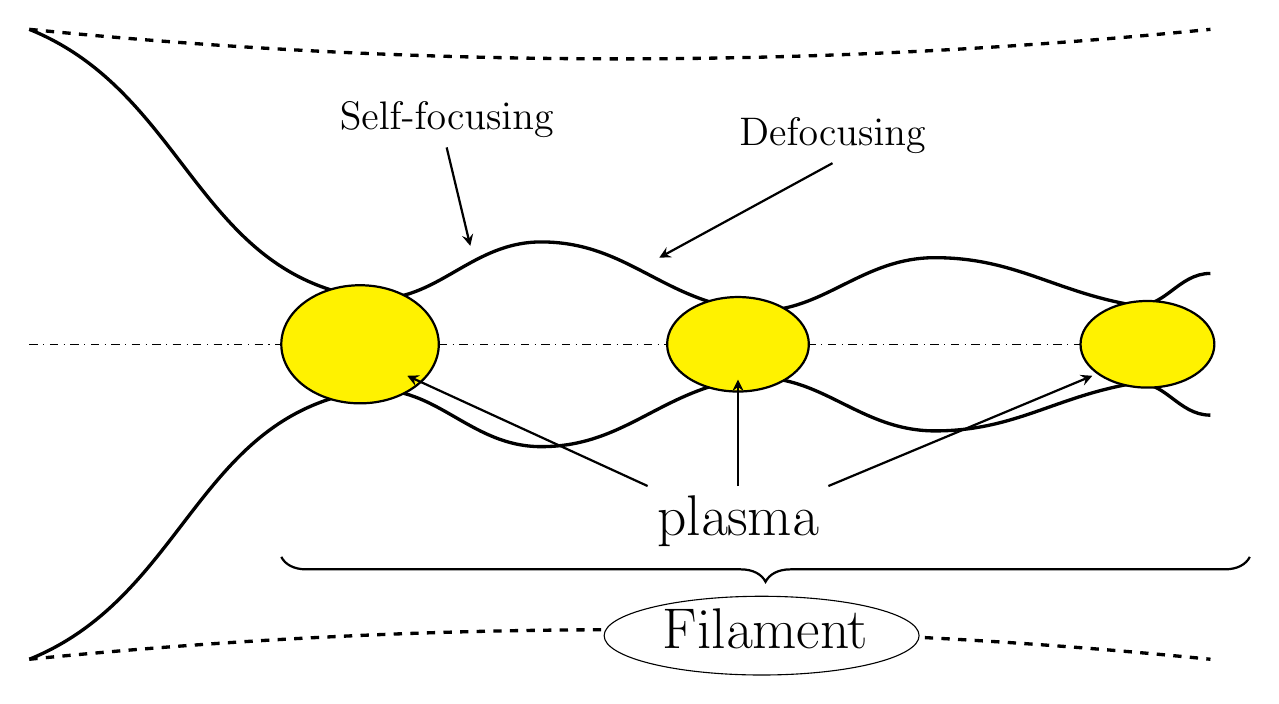
\begin{tikzpicture}[>=stealth]
        \def\xend{15}
        \def\ymax{4}

        \draw[dash dot, thin] (0,0) -- (\xend,0) [->];

        \draw[very thick, dashed] (0, \ymax) .. controls (5, 3.5) and (10, 3.5) .. (\xend, \ymax);
        \draw[very thick, dashed] (0, -\ymax) .. controls (5, -3.5) and (10, -3.5) .. (\xend, -\ymax);

        \draw[very thick] (0, \ymax)
            to[out=-22, in=170] (4.2, 0.6)
            to[out=-10, in=180] (6.5, 1.3)
            to[out=0, in=170]   (9.0, 0.45)
            to[out=-10, in=180] (11.5, 1.1)
            to[out=0, in=170]   (14.0, 0.5)
            to[out=-10, in=180] (\xend, 0.9);

        \draw[very thick] (0, -\ymax)
            to[out=22, in=-170] (4.2, -0.6)
            to[out=10, in=-180] (6.5, -1.3)
            to[out=0, in=-170]  (9.0, -0.45)
            to[out=10, in=-180] (11.5, -1.1)
            to[out=0, in=-170]  (14.0, -0.5)
            to[out=10, in=-180] (\xend, -0.9);
        \draw[fill=white] (9.3, -3.7 ) ellipse (2 and 0.50);
        \draw[fill=yellow, thick] (4.2, 0) ellipse (1.0 and 0.75);
        \draw[fill=yellow, thick] (9.0, 0) ellipse (0.9 and 0.6);
        \draw[fill=yellow, thick] (14.2, 0) ellipse (0.85 and 0.55);

        \node[above] (sf) at (5.3, 2.5) {\Large Self-focusing};
        \draw[->, thick] (sf.south) -- (5.6, 1.25);

        \node[above] (df) at (10.2, 2.3) {\Large Defocusing};
        \draw[->, thick] (df.south) -- (8.0, 1.1);

        \node[below] (plasma_text) at (9.0, -1.8) {\huge plasma};
        \draw[->, thick] (plasma_text.north west) -- (4.8, -0.4);
        \draw[->, thick] (plasma_text.north) -- (9.0, -0.45);
        \draw[->, thick] (plasma_text.north east) -- (13.5, -0.4);

        \draw[decorate, decoration={brace, amplitude=9pt, mirror}, thick]
            (3.2, -2.7) -- (15.5, -2.7) node[midway, below=15pt] {\huge Filament};
    \end{tikzpicture}%
    }
    \caption{Schematic beam envelope undergoing repeated cycles of Kerr self-focusing and plasma defocusing. Each collapse is arrested before catastrophic self-focusing by the free electron plasma generated near the intensity peak (yellow), which defocuses the beam until the intensity drops enough for the plasma to recombine and self-focusing to take over again, refilled by the surrounding energy reservoir. This repeated breathing over an extended propagation distance is the filament.}
    \label{fig:filamentation_schematic}
\end{figure}


The critical power $P_{cr}$ follows from the balance between the nonlinear self-focusing effect and diffraction. For a Gaussian beam, it is given by~\cite{marburger1975}:
\begin{equation}
    P_{cr} = \frac{3.77 \lambda_0^2}{8 \pi n_0 n_2},
\end{equation}
where $\lambda_0$ is the laser wavelength, $n_0$ the linear refractive index, and $n_2$ the nonlinear index coefficient. The numerical factor is $3.77$ for a Gaussian beam and $3.72$ for the Townes profile, for which diffraction and self-focusing balance exactly.

Above threshold, the distance at which an unopposed beam would collapse is given by the semi-empirical formula fitted to numerical solutions of the nonlinear Schr\"odinger equation by Dawes and Marburger~\cite{dawes1969,marburger1975}:
\begin{equation}
    \label{eq:marburger}
    L_c = \frac{0.367\, L_{DF}}{\sqrt{\big[(P_{in}/P_{cr})^{1/2} - 0.852\big]^2 - 0.0219}},
\end{equation}
where $L_{DF} = k_0 w_0^2 / 2$ is the Rayleigh length. For an externally focused beam of focal length $f$, the collapse distance shortens according to $L_{c,f}^{-1} = L_c^{-1} + f^{-1}$. Equation~\eqref{eq:marburger} is what sets the position of the nonlinear focus in the simulations, before plasma defocusing arrests the collapse.

For fused silica, typical values at $\lambda_0 = 800 \text{ nm}$ are $n_0 \approx 1.45$ and $n_2 \approx 2.4 \times 10^{-20} \text{ m}^2/\text{W}$, a value measured by Taylor et al. and reported in the reference compilation of Milam~\cite{milam1998}. Using these values, we calculate $P_{cr} \approx 2.8 \text{ MW}$, consistent with the $1.98$ to $2.5\text{ MW}$ reported respectively in~\cite{PhysRevB.71.125435} and~\cite{kandidov2009} for fused silica at this wavelength. At $\lambda_0 = 1030 \text{ nm}$, since no measurement exists exactly at this wavelength, we use the closest value available in the literature, $n_2 \approx 2.74 \times 10^{-20} \text{ m}^2/\text{W}$ at $1053\text{ nm}$~\cite{milam1998}, which gives $P_{cr} \approx 4.0 \text{ MW}$.

The critical power is related to the laser intensity $I$ through the beam cross section. For a Gaussian beam of radius $w_0$, the peak intensity is:
\begin{equation}
    I_0 = \frac{2 P}{\pi w_0^2}.
\end{equation}

In the tight focusing experiments of~\cite{PhysRevB.71.125435}, the measured beam radius at focus ranges from $0.7$ to $4.8\ \mu$m depending on the objective used, with $w_0 = 1.1\ \mu$m for the $20\times$, NA $=0.5$ objective retained in that reference. Taking this radius with $P = P_{cr} \approx 2.8\text{ MW}$, we obtain an intensity of order $1.5 \times 10^{14} \text{ W/cm}^2$, higher than the clamping intensity of about $5 \times 10^{13} \text{ W/cm}^2$ actually measured in~\cite{PhysRevB.71.125435}. This gap is expected. $I_0 = 2P/(\pi w_0^2)$ assumes linear focusing all the way down to the radius $w_0$, whereas in reality the defocusing produced by the plasma generated during propagation limits the peak intensity well before the beam reaches this radius, which is why the observed clamping intensity remains lower than this simple geometric estimate.


\begin{figure}[htbp]
    \centering
    \begin{subfigure}{0.49\textwidth}
        \centering
        
\includegraphics[width=\linewidth]{fig7a_fluence_045uJ.png}
        \caption{$0.45\ \mu$J.}
    \end{subfigure}
    \hfill
    \begin{subfigure}{0.49\textwidth}
        \centering
        
\includegraphics[width=\linewidth]{fig7b_fluence_11uJ.png}
        \caption{$1.1\ \mu$J.}
    \end{subfigure}
    \caption{Fluence contours (solid black, in $\text{J/cm}^2$) and beam radius at half maximum (dashed blue) along the propagation axis, reproducing Fig.~7 of~\cite{PhysRevB.71.125435} at $800\ \text{nm}$, $160\ \text{fs}$, for two input pulse energies. At $0.45\ \mu$J the beam radius pinches once around the nonlinear focus and re-expands, the single self-focusing/defocusing cycle of Fig.~\ref{fig:filamentation_schematic}. At $1.1\ \mu$J, above threshold by a larger margin, the pinch splits into two separate foci with a secondary local waist further downstream, a second refocusing cycle fed by the surrounding energy reservoir, consistent with the multiple-cycle picture of Section~1.3.12 of the Couairon review.}
    \label{fig:fig7_fluence_contours}
\end{figure}

\begin{figure}[htbp]
    \centering
    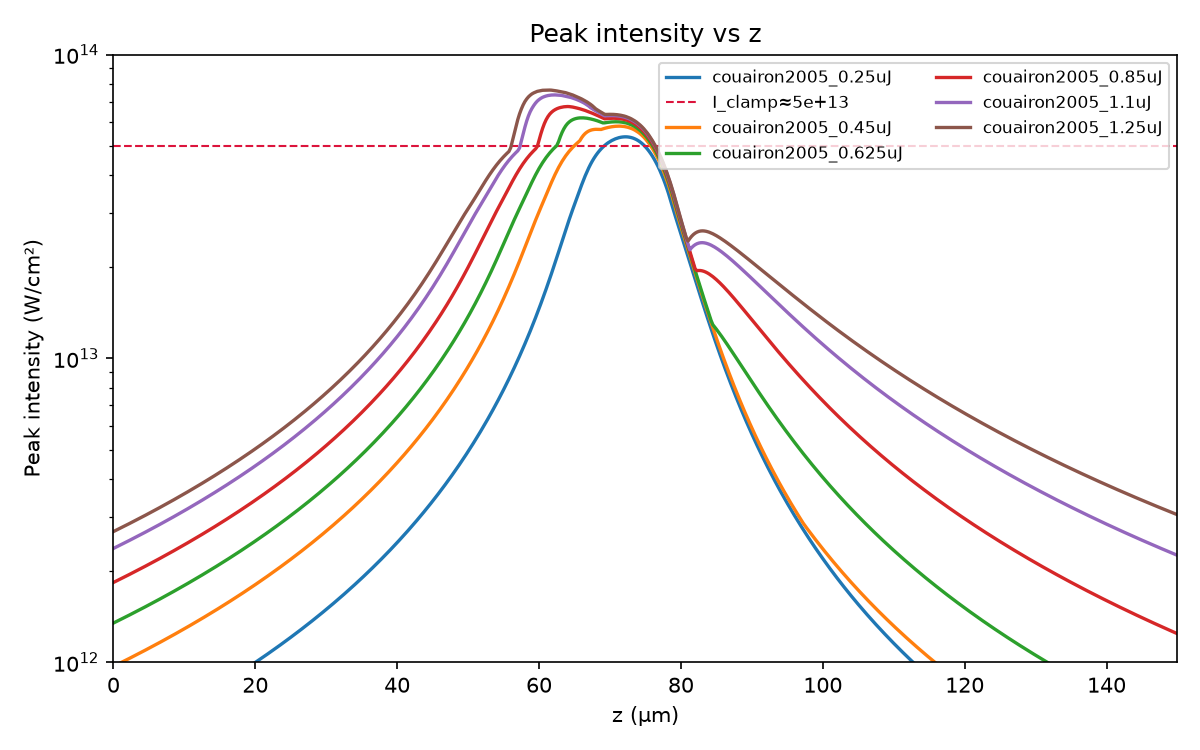
\includegraphics[width=0.85\linewidth]{couairon2005_fig8_energy_sweep.png}
    \caption{Peak on-axis intensity along $z$ for six input pulse energies from $0.25$ to $1.25\ \mu$J, reproducing Fig.~8 of~\cite{PhysRevB.71.125435}. Below threshold the peak intensity simply follows linear focusing (lower curves never reach $I_{clamp}$). Above it, every curve saturates at essentially the same value close to the clamping intensity $I_{clamp}\approx5\times10^{13}\ \text{W/cm}^2$ (dashed line) predicted from the intensity-clamping balance of Section~1.3.4 of the Couairon notes, before decaying on the trailing side of the nonlinear focus. This saturation, common to all above-threshold energies despite their different $P_{in}/P_{cr}$ ratios, is the numerical signature of intensity clamping referred to throughout Section~8.2.}
    \label{fig:fig8_peak_intensity}
\end{figure}

\FloatBarrier
\subsection{Cross-Validation Against Independent Simulations}

The figures above reproduce the specific published results of~\cite{PhysRevB.71.125435} at their exact laser parameters, as a check that the solver reproduces a result it was not tuned against. This subsection adds two further independent checks: a second published simulation with an entirely different parametrization, and an ablation of the propagation equation itself on the experiment actually used throughout this report.

\begin{figure}[htbp]
    \centering
    
\includegraphics[width=0.95\linewidth]{fig11.png}
    \caption{Fluence, absorbed energy density, peak intensity and electron density maps for the conditions of Bulgakova, Stoian \& Rosenfeld ($800\ \text{nm}$, $120\ \text{fs}$, $1\ \mu$J, $w_0=0.9\ \mu$m, geometric focus at $90\ \mu$m below the surface, dashed white line), a parametrization independent of~\cite{PhysRevB.71.125435} (different $n_2$, effective mass, collision time and lattice density). White contours mark the levels published in that reference; the solver's own fields (colour maps) fall within them across all four panels, including the secondary lobe past the geometric focus visible in panels (a)-(c), itself a signature of the refocusing cycle of Fig.~\ref{fig:filamentation_schematic}.}
    \label{fig:bulgakova_fig11}
\end{figure}

\begin{figure}[htbp]
    \centering
    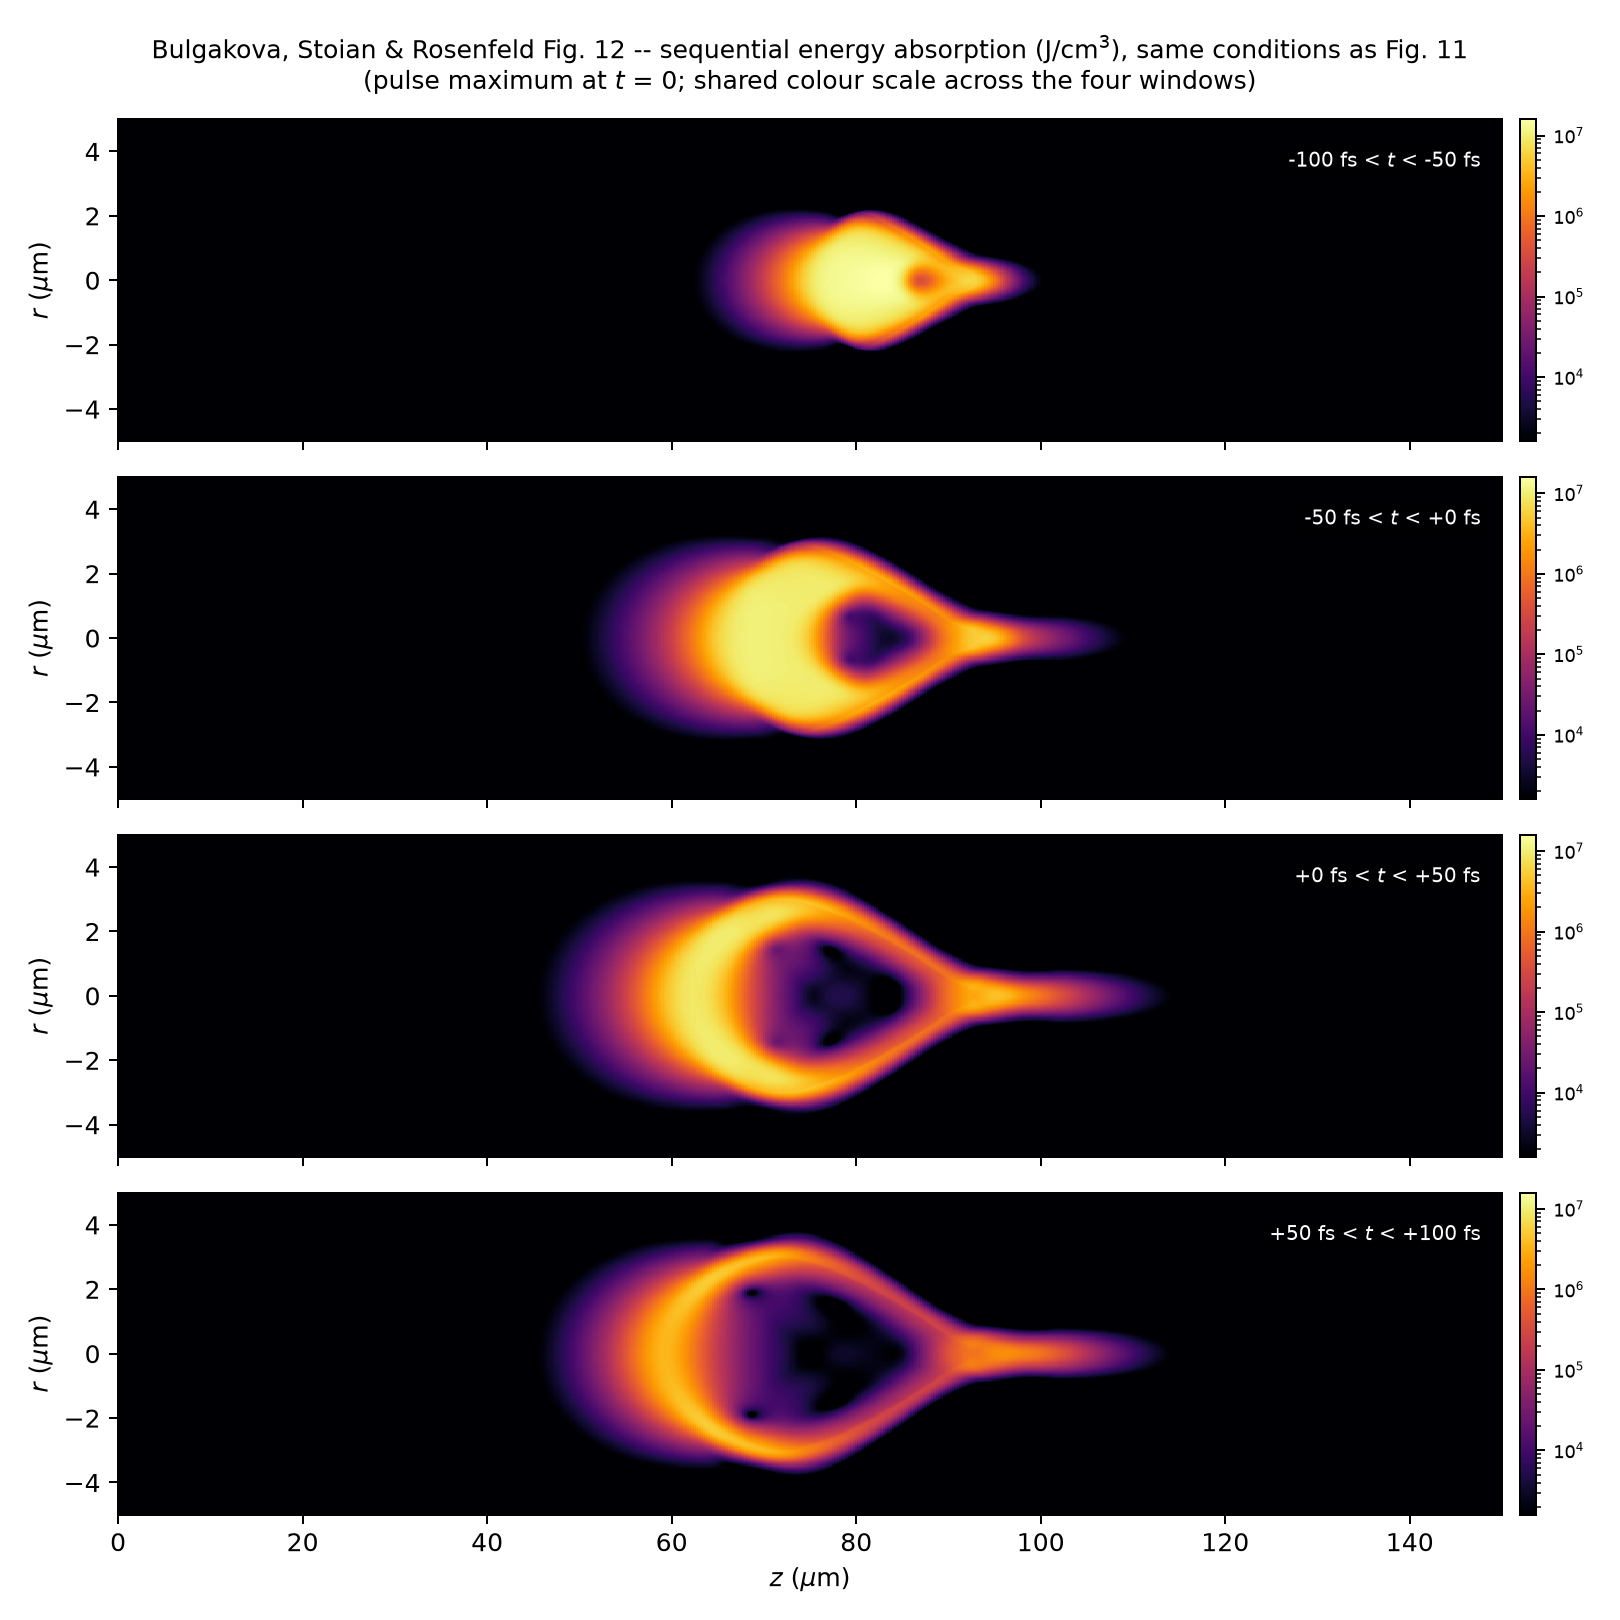
\includegraphics[width=0.95\linewidth]{fig12.png}
    \caption{Energy absorbed in four successive $50\ \text{fs}$ windows of the same pulse as Fig.~\ref{fig:bulgakova_fig11}, on a shared colour scale. Absorption is confined to a compact region near the pulse peak in the first window, then spreads into a hollow, ring-shaped pattern reaching further upstream (toward smaller $z$) in the later windows, consistent with plasma generated earlier in the pulse pre-absorbing and defocusing the beam before it reaches material deeper along the propagation axis.}
    \label{fig:bulgakova_fig12}
\end{figure}

\begin{figure}[htbp]
    \centering
    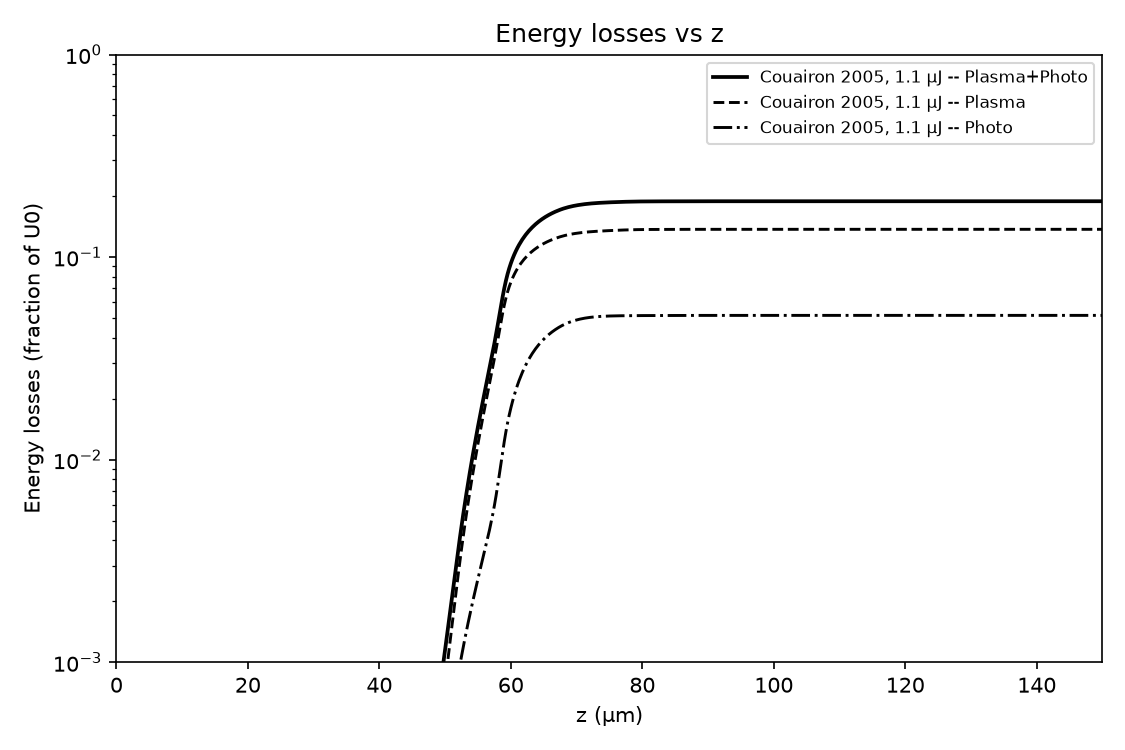
\includegraphics[width=0.8\linewidth]{fig12_energy_losses.png}
    \caption{Cumulative energy lost by the pulse of~\cite{PhysRevB.71.125435} (at $1.1\ \mu$J) as it propagates, as a fraction of the input energy $U_0$, separated into the plasma absorption and photoionization channels. Both losses turn on together at the nonlinear focus and saturate once the beam has defocused past the clamping intensity, plasma absorption (inverse bremsstrahlung on already-free carriers) accounting for roughly $2.5\times$ more of the total loss than direct photoionization, consistent with the two channels' relative weight, $\sigma_\omega/U_i$ against $W_{PI}/\rho_{at}$, discussed in Section~4.}
    \label{fig:energy_losses}
\end{figure}

\begin{figure}[htbp]
    \centering
    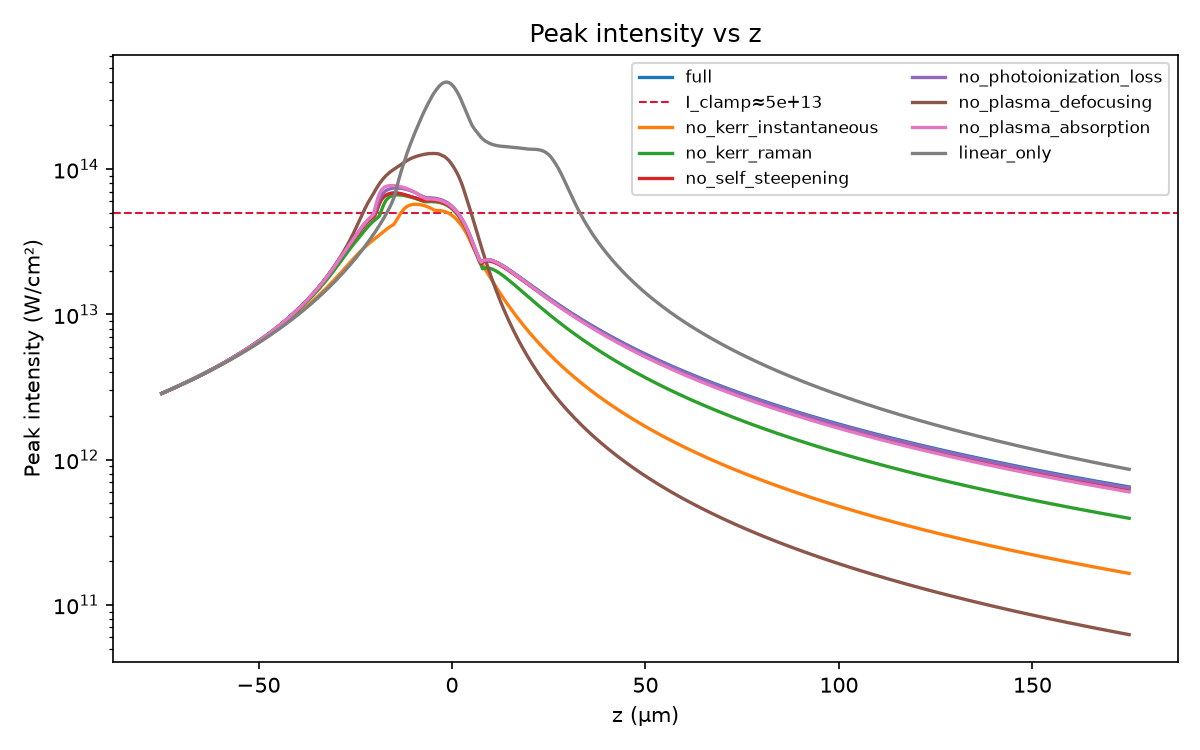
\includegraphics[width=0.85\linewidth]{comparison_fig8_peak_intensity.png}
    \caption{Peak on-axis intensity along $z$ for the experiment actually used throughout this report ($1030\ \text{nm}$, $263\ \text{fs}$, $15\ \mu$J, self-trapped exciton channel active), with each physical term of Eq.~\eqref{eq:master_propagation} disabled in turn. \texttt{linear\_only} (pure diffraction and dispersion, no Kerr, no plasma) overshoots the clamping intensity by nearly an order of magnitude, confirming that the balance discussed in Section~8.1 is what limits the intensity in every other curve. \texttt{no\_plasma\_defocusing} keeps the ionization losses but removes the defocusing phase, and reaches roughly twice the clamping intensity before the accumulated photoionization and avalanche losses alone eventually arrest it, showing that defocusing, not absorption, does most of the clamping work. \texttt{no\_kerr\_instantaneous} and \texttt{no\_kerr\_raman} both peak lower than \texttt{full} and decay markedly faster past the nonlinear focus, roughly an order of magnitude below \texttt{full} by $z=150\ \mu$m, consistent with the weaker Kerr response lengthening $L_c$ of Eq.~\eqref{eq:marburger}. The remaining curves (no self-steepening, no photoionization loss, no plasma absorption) are visually indistinguishable from \texttt{full} at this scale, since none of them changes the dominant balance between Kerr self-focusing and plasma defocusing that sets the clamping intensity itself.}
    \label{fig:comparison_fig8}
\end{figure}
\FloatBarrier

\subsection{Exciton Formation}

When an electron is promoted from the valence band to the conduction band, for example by optical absorption, it leaves behind a hole of effective charge $+e$. Electrons in the conduction band can feel the potential created by the holes in the valence band. This electrostatic attraction can be modeled by a Coulomb potential, which allows us to solve the Schrödinger equation for a composite particle called an \textbf{exciton}, made of a conduction band electron and a valence band hole.

This quasiparticle has a reduced mass defined by $\frac{1}{\mu} = \frac{1}{m_e} + \frac{1}{m_h}$ and a quantized energy spectrum of the hydrogen-like type.

In the absence of Coulomb interaction, the minimum energy required to create a free electron-hole pair corresponds to the gap energy $E_g$. However, because of the attractive Coulomb potential between the electron and the hole, they can form a bound state. The accessible energy levels then sit below the conduction band. These states can be populated directly through the process described above, but also through nonradiative relaxation mechanisms such as the Auger effect or exciton-phonon interactions. As pointed out by Mao et al.~\cite{mao2004}, this formation process is very fast, often under $1 \text{ ps}$ for wide bandgap materials.

The relative motion of this electron-hole pair can be modeled by a hydrogen-like Schrödinger equation. The stationary equation for the relative coordinate $\mathbf{r}$ reads:
\begin{equation}
    \left[ \frac{\hbar^2}{2\mu} \nabla^2 + \frac{e^2}{4\pi \epsilon_0 \epsilon_r r} \right] \psi(\mathbf{r}) = E_b \psi(\mathbf{r}),
\end{equation}
where $\epsilon = \epsilon_0 \epsilon_r$ is the dielectric permittivity of the medium and $E_b > 0$ is the exciton binding energy.

The relation between the gap energy $E_g$, the binding energy term, and the excitation energy $E_n$ required for the $n$-th exciton state is given by:
\begin{equation}
    E_g = E_n + \frac{R_\chi}{n^2},
\end{equation}
where $R_\chi$ is the effective exciton Rydberg energy:
\begin{equation}
    R_\chi = \frac{\mu e^4}{2(4\pi \epsilon)^2 \hbar^2} = R_H \left(\frac{\mu}{m_0}\right) \frac{1}{\epsilon_r^2}.
\end{equation}
Here, $R_H \approx 13.6\text{ eV}$ is the Rydberg constant of the hydrogen atom, $m_0$ is the free electron mass, and $\epsilon_r$ is the relative dielectric constant of the material.

To evaluate the spatial extent of the exciton wavefunction, we define the exciton Bohr radius $a_\chi$:
\begin{equation}
    a_\chi = \frac{4\pi \epsilon \hbar^2}{\mu e^2} = a_0 \cdot \epsilon_r \left(\frac{m_0}{\mu}\right),
\end{equation}
where $a_0 \approx 0.53\text{ \AA}$ is the atomic Bohr radius.

In wide bandgap materials, electrons are strongly bound to their atoms, which means the relative dielectric permittivity is low for $\mathrm{SiO}_2$ or alkali halides, where the relative dielectric constant is typically of order $2$ to $4$. As a result, the material provides weak dielectric screening of the Coulomb attraction, maintaining a deep potential well.

A low permittivity directly leads to a reduction of the exciton Bohr radius, down to a few angstroms. When $a_\chi$ becomes comparable to the interatomic spacing of the lattice, the exciton localization no longer extends over several lattice atoms but shifts to a strongly bound regime. The binding energy also increases, preventing thermal dissociation and favoring ultrafast energy relaxation. During this process, the excess electrostatic potential energy of the unscreened exciton is abruptly discharged into local lattice vibrations (phonons) through massive exciton-phonon coupling within a few picoseconds. This induces a local lattice distortion and leads to the formation of a self-trapped exciton (STE).

\subsection{Self-Trapped Excitons}

Thermal fluctuations induce slight lattice vibrations that act as a trigger, creating a transient local deformation. The strongly localized exciton is captured by this distortion. Through massive exciton-phonon coupling, it abruptly discharges its potential energy into the lattice, considerably deepening the local potential well.

This intense localized energy weakens and breaks the $\text{Si--O--Si}$ covalent bond, displacing the oxygen atom from its equilibrium position. This structural rupture generates two dangling bonds, each holding an unpaired electron. In this strongly distorted configuration, the exciton self-traps. The hole localizes on the oxygen dangling bond, while the electron remains bound to the silicon dangling bond~\cite{mao2004}.

This mechanism explains the formation of \textbf{Self-Trapped Excitons} (STE) in silica, where the excitation energy is rapidly converted into local lattice distortion, opening the way to permanent structural modifications of the material~\cite{mao2004}.


\begin{thebibliography}{9}

\bibitem{fork1981}
R. L. Fork, B. I. Greene, and C. V. Shank,
\textit{Generation of optical pulses shorter than 0.1 psec by colliding pulse mode locking},
Appl. Phys. Lett. (1981).

\bibitem{zewail1994}
A.H. Zewail, 
\textit{Femtochemistry: Ultrafast Dynamics of the Chemical Bond},
World Scientific, Singapore (1994).

\bibitem{shah1996}
J. Shah, 
\textit{Ultrafast Spectroscopy of Semiconductors and Semiconductor Nanostructures},
Springer, Berlin Heidelberg New York (1996).

\bibitem{mao2004}
S.S. Mao et al.,
\textit{Dynamics of femtosecond laser interactions with dielectrics},
Appl. Phys. A 79, 1695–1709 (2004).

\bibitem{bulgakova2010}
N.M. Bulgakova, R. Stoian, A. Rosenfeld,
\textit{Laser-induced modification of transparent crystals and glasses},
Quantum Electron. 40 966 (2010).

\end{thebibliography}


\end{document}
